\documentclass[12pt,a4paper]{article}
\usepackage[utf8]{inputenc}
\usepackage{amsmath}
\usepackage{amsfonts}
\usepackage{amssymb}
\usepackage{graphicx} % for figure
\usepackage[font=footnotesize]{caption}
\usepackage{subcaption}  % for subfigure
\usepackage{float}
\usepackage{indentfirst} % indent first line after section title
\usepackage{placeins} %FloatBarrier
\usepackage{afterpage}

\author{Joao Guilherme Caldas Steinstraesser \\ José Galaz}
\title{Inriamericwaves \\ Report of activities - March-May/16}

\bibliographystyle{abbrv}

\captionsetup[subfigure]{labelformat=parens,labelsep=space}

%% Commands
\newcommand{\der}[1]{\partial_{#1}}
\renewcommand{\epsilon}{\varepsilon}

\renewcommand{\th}{\tilde{h}}
\newcommand{\tu}{\tilde{u}}

\newcommand{\lh}{\overline{h}}
\newcommand{\lu}{\overline{u}}

\newcommand{\opT}{\mathcal{T}}
\newcommand{\opQ}{\mathcal{Q}}
\newcommand{\opIT}{I + \opT}
\newcommand{\opIhT}{I + h\opT\frac{1}{h}}

\newcommand{\Atwo}[2]{\left( \begin{array}{c} #1 \\ #2  \end{array} \right)}

\begin{document}
\maketitle

\newpage
\tableofcontents

\newpage
\section{Introduction}

\indent L'objectif de l'adaptation de maillages développée dans ce stage est de modifier la position de ses noeuds par rapport à une fonction donnée, ou à une solution d'un problème physique, de façon qu'on puisse avoir un raffinement variable au long du domaine et qui représente bien la présence de fortes gradients, surfaces, etc., sans modifier le nombre de points ni la connectivité du maillage.

\indent Dans ce rapport, on va présenter dans un premier moment l'application de l'algorithme à l'adaptation à des fonctions Level Set, à fin d'obtenir une bonne représentation d'un objet. Cette fonction, définie pour tout point du maillage, est la distance signée entre le point et l'objet, où la signe indique s'il est à son intérieur ou extérieur \cite{ducrot}. Ainsi, la ligne de niveau 0 de la fonction Level Set représente la surface de l'objet, et on utilisera ce fait pour orienter l'adaptation du maillage.

\indent Ensuite, on résoudra des problèmes de la mécanique des fluides sur les maillages adaptés et, avec les résultats obtenus, on fera des nouvelles adaptations, mais cette fois-ci en utilisant au même temps la fonction Level Set et la solution physique du problème. Avec cette procédure, on sera capable d'obtenir des maillages encore plus appropriées au calcul envisagé. 

\indent Le rapport est organisé de la façon suivante : dans la section \ref{sec:modele}, on va d'abord présenter, de façon plus générale, le modèle utilisé pour l'adaptation de maillages, selon la formulation développée par \cite{arpaia}, et des détails concernant son implémentation. L'application du modèle à l'adaptation à des fonctions Level Set sera décrite dans la section \ref{sec:application}, avec quelques exemples de tests réalisés et une indication des paramètres qui ont produit les meilleurs résultats. Le couplage avec l'adaptation physique et les résultats obtenus sont présentés dans la section \ref{sec:adapPhysique}. Enfin, dans la section \ref{sec:nonstat}, on utilise le modèle pour adapter le maillage à des objets en mouvement. Par ailleurs, on remarque que la plupart du contenu de ce rapport se réfère à des cas 2D; pourtant, nous présentons aussi quelques résultats pour des exemples 3D.

\indent Les exemples présentés dans ce rapport ne sont qu'une petite partie de l'ensemble des tests réalisées  au cours de ce stage. Ces tests ont eu une grande importance pour valider, corriger et développer le modèle,  tester la bibliothèque et les plusieurs parties du code, et trouver les paramètres et stratégies d'adaptation qui nous permettent d'obtenir les meilleurs résultats en tenant compte des objectifs décrits ci-dessus. La section \ref{sec:autres} présente une liste des rapports rédigées pour décrire et présenter ces tests.
\section{KdV equation}
\label{sec:KdV}

\subsection{The model}

\indent The first model of wave propagation studied and implemented in this project is the Korteweg-de Bries (KdV) equation, which takes in account  nonlinear and dispersive effects and is a good approximation for waves with small amplitude and long wavelength.

\indent Different forms of this equation can be found in literature, varying mainly in the scaling factors for each physical process present in the equation (nonlinearity and dispersion). We will consider the formulation derived by \cite{BBM1971}, written in terms of dimensionless but unscaled variables :

\begin{equation}
    u_t + u_x + (u^2)_x + u_{xxx} = 0
\end{equation}

\subsection{Discretization}

\indent The problem to be solved, with a initial condition $\Phi$ and proper boundary conditions, is

\begin{equation}
\begin{cases}
    u_t + u_x + (u^2)_x + u_{xxx} = 0 \ , \ \ x \in [x_{min},x_{max}], \ \ t \in [0, t_{max}] \\
    u(x,0) = \Phi(x) \\
    \text{+ boundary conditions}
\end{cases}
\end{equation}

\indent In a first moment, in order to validate the implementation of the model, without influence of the boundaries, we will consider periodic boundary conditions or, in the nonperiodic case, homogeneous Dirichlet and/or Neumann conditions with the boundaries far enough from the propagating wave.

\indent The numerical resolution will be made with a splitting scheme, separating the advective and the dispersive terms. Therefore, defining the operators


\begin{gather}
	T_a{u} = u_t + u_x + (u^2)_x \\
	T_d{u} = u_t + u_{xxx}
\end{gather}

 
\noindent we will solve, in each time step $[t_n,t_{n+1}]$ :

\begin{equation}
\begin{cases}
   T_a(v) = 0 \ \ ,\ t \in [t_n,t_{n+1}], \  v^n = u^n \\
   T_d(w) = 0 \ \ , \ t \in [t_n,t_{n+1}], \  w^n = v^{n+1} \\
    u^{n+1} = w^{n+1}
\end{cases}
\end{equation}

\indent The numerical schemes used in each of these step is descried below :

\subsubsection{First step}
\label{sec:KdVSplitted1}

\indent The first step of the splitted KdV equation is a hyperbolic conservation law, which can be written in terms of a flux function $f$ :

\begin{equation}
  \label{eq:conservationLaw}
	v_t + f(v)_x = 0, \ \ f(v) = v + v^2
\end{equation}

\indent It will be solved using a Finite Volume method, with the cells $[x_{i-1/2}, x_{i+1/2}]$ centered in the discrete spatial points $x_i$ and with the cell-averaged value of the solution equal to the solution $u_i^n$ in these points. The spatial derivative in \eqref{eq:conservationLaw} will be discretized with a 4th order Runge-Kutta method,

\begin{equation}
\begin{cases}
k_1 = - f(v_i^n)_x \\
k_2 = - f\left(v_i^n + k_1\frac{\Delta t }{2}\right)_x \\
k_3 = - f\left(v_i^n + k_2\frac{\Delta t }{2}\right)_x \\
k_4 = - f(v_i^n + k_3 \Delta t)_x \\
v_i^{n+1} = v_i^n + \frac{\Delta t}{6}(k_1 + 2k_2 + 2k_3 + k_4)
\end{cases}
\end{equation}

\noindent and the spatial derivative will be approximated in terms of the flux on the cells' interfaces : 

\begin{equation}
f(v_i^n)_x = \frac{f\left(v_{i+1/2}^n\right) - f\left(v_{i-1/2}^n\right)}{\Delta x}
\end{equation}

\indent Therefore, we must compute the values of $u$ on each interface. It will be made solving the following Riemann problem :

\begin{equation}
\begin{cases}
v_t + f(v)_x = 0 \\
v(x,0) = v^- \ , \ x < 0 \\
v(x,0) = v^+ \ , \ x > 0
\end{cases}
\end{equation}

\noindent where the boundary is located at $x=0$ and $v^-$ and $v^+$ are the solutions in its two neighbor cells.

\indent The flux function $f$ is uniformly convex, so the Riemann problem has a unique weak, admissible solution \cite{conservationLaws2002} : 

\begin{itemize}
\item  If $v^- > v^+$  (shock) : 
\begin{equation}
v(x,t) = 
\begin{cases}
v^- \ ,\ \   f(v^-) > f(v^+) \\
v^+ \ ,\ \ f(v^-) < f(v^+)
\end{cases}
\end{equation}

\item If $v^+ > v^-$  (rarefaction wave) :
\begin{equation}
v(x,t) = 
\begin{cases}
v^- \ ,\ \ f'(v^-) > 0 \\
\left(f'\right)^{-1}(v) \ ,\ \ f'(v^-) < 0 < f'(v^+) \\
v^+ \ ,\ \ f'(v^+) < 0 
\end{cases}
\end{equation}
\end{itemize}


\subsubsection{Second step}

\indent Two schemes will be proposed for the resolution of the second step of the KdV equation,

\begin{equation}
	\label{eq:dispersion}
	w_t + w_{xxx} = 0
\end{equation}

\noindent depending on the boundary conditions (periodic or not).

\paragraph{Periodic case}

\indent The spatial derivatives and the linearity in the second step \eqref{eq:dispersion} motivates us to implement a Fourier spectral method, which is possible with the periodic boundary conditions. In fact, the method is quite simple :

\indent Let $\hat{w}(k,t_n)$ be the Fourier coefficients of $w(x,t_n)$.  The Fourier transform of the equation \eqref{eq:dispersion} gives

\begin{equation}
	\hat{w}_t(k,t) - ik^3\hat{w}(k,t) = 0
\end{equation}

\indent It is an ODE in $t$,  which solution is

\begin{equation}
\hat{w}(k,t) = e^{ik^3(t-t_n)}\hat{w}(k,t_n)
\end{equation}

\indent Finally, the inverse Fourier transform using the coefficients $\hat{w}(k,t_{n+1})$ gives $w(x,t_{n+1})$

\paragraph{Nonperiodic case}

\indent For this case, the second equation \eqref{eq:dispersion} was solved using an implicit Finite Difference scheme, with fourth order centered discretization of the third spatial derivative, except in the points near the boundaries, for which a simple first order uncentered scheme was used:

\begin{gather}
	\label{eq:IFDSolverKdV}
	\frac{u_i^{n+1} - u_i^n}{\Delta t} + \frac{\frac{1}{8}u_{i-3}^{n+1} - u_{i-2}^{n+1}  + \frac{13}{8}u_{i-1}^{n+1} - \frac{13}{8}u_{i+1}^{n+1} + u_{i+2}^{n+1} - \frac{1}{8}u_{i+3}^{n+1}}{\Delta x^3} = 0, \ \ i = 3,...,N-3 \\
	\frac{u_i^{n+1} - u_i^n}{\Delta t}  + \frac{-u_{i}^{n+1} + 3u_{i+1}^{n+1}  -3 u_{i+2}^{n+1} + u_{i+3}^{n+1} }{\Delta x^3} = 0, \ \ i = 0,1,2 \\
	\frac{u_i^{n+1} - u_i^n}{\Delta t}  + \frac{u_{i}^{n+1} - 3u_{i-1}^{n+1}  + 3 u_{i-2}^{n+1} - u_{i-3}^{n+1} }{\Delta x^3} = 0, \ \ i = N-2,N-1,N \\
\end{gather} 

\noindent which leads to the resolution of a linear system, with the appropriate modifications to take in account the boundary conditions.

\subsubsection{Choice of the time step}

\indent The time step is chosen based on the first step of the splitted equation. In the non-conservative form, the equation \eqref{eq:conservationLaw} is written as

\begin{equation}
v_t +  (1+2v)v_x = 0
\end{equation}

\noindent which configures an advection problem with velocity $1+2v$

\indent The space and time steps must verify the CFL condition : 

\begin{equation}
(1+2v)\frac{\Delta t}{\Delta x} \leq 1
\end{equation}

\noindent in order to avoid non-physical behaviors (e.g. mass increasing). Therefore, for each time step, we will chose, for small $\epsilon$

\begin{equation}
\Delta t = \frac{\Delta x}{1+2\max\limits_{x}|v|} - \epsilon
\end{equation}

\subsection{Scale analysis}

\indent With the objectif of correctly simulating the physical phenomena involved in the KdV equation, the initial solution must satisfy the assumptions made in the derivation of the model. Following this purpose, we perform in the next paragraphs a scale analysis following the arguments presented in \cite{BBM1971}, which at the same time will be linked to the physical case of water surface waves of small amplitude. This analysis will allow us to derive a criteria for selecting the initial conditions of some example simulations. 

\indent We will seek to write the KdV equation in the following dimensionless and scaled form, as described in \cite{BBM1971}

\begin{equation}
\label{eq:scaledKdV}
U_T + U_X + \frac{\epsilon}{2} (U^2)_X + \epsilon\alpha^2U_{XXX} = 0
\end{equation}

\noindent and link it to the parameters involved in the model for surface water waves  in dimensional form \cite{Khorsand2014}

\begin{equation}
    u^*_{t^*} + c_0u^*_{x^*} + \frac{3}{4}\frac{c_0}{h_0}({u^*}^2)_{x^*} + \frac{1}{6}c_0h_0^2u^*_{x^*x^*x^*} = 0 
\end{equation}

\noindent where the $\cdot^*$ denotes the physical variables, $h_0$ the undisturbed water depth for flat bottom and $c_0 = \sqrt{gh_0}$  the long wave speed.

\subsubsection{Characterization of the nonlinearity}

\indent According to \cite{BBM1971}, nonlinearity is characterized by a parameter $\epsilon$ such that if characteristics are written in the form

$$ \frac{1}{c_0} \frac{dx}{dt} = 1+ bu$$

\noindent then one can choose an $\epsilon \ll 1$ such that $bu=\epsilon U$, with $U$ of order one. For the particular case of water waves this can be represented as

$$ \frac{1}{c_0} \frac{dx}{dt} = 1 + \frac{3}{2h_0}u$$

\noindent and thus $b = \frac{3}{2h_0}$. This parameter will be used in the next arguments.

\subsubsection{Characterization of the dispersion}

\noindent The characterization of the dispersion comes from the derivation of the KdV equation. According to \cite{BBM1971} if the propagation of the wave follows a law of the form

$$ u^*_{t^*} + uu_x+(\mathcal{L} u^*)_{x^*} = 0$$

\noindent with $\mathcal{L}$ such that $$ \widehat{\mathcal{L}u^*} = \frac{c(k)}{c_0} \widehat{u^*}(k,t)$$ with $\hat \cdot$ the Fourier transform and $c(k)$ the phase celerity, which is equivalent to 

$$ \mathcal{L} u = \mathcal{F}^{-1}\left(\frac{c(k)}{c_0}\right) * u$$ 

\noindent where $\mathcal{F}^{-1}$ is the inverse Fourier transform operator, then new scaling based on the fact that for $\kappa$ sufficiently small, the wave speed $c(\kappa) = c_0 + c_0 \sum_{n=1}^{\infty}A_n\epsilon^n\kappa^{2n}$ can be approximated by $c(\kappa) = c_0(1-\kappa^2)$, which motivates replacing $x=\sqrt{\epsilon} X$, $t =c_0 \sqrt{\epsilon} T$, and $u = \frac{\epsilon}{ b} U$ to obtain the equivalent equation 

$$ U_T + \epsilon U U_x+(\mathcal{L}_{\epsilon} U)_{X} = 0$$

\noindent with $\mathcal{L}_\epsilon$ such that 

$$ \widehat{\mathcal{L}_\epsilon U} = \frac{c(\epsilon^{1/2} K)}{c_0} \hat{U}(K,T)$$ 

\noindent with $K=\sqrt{\epsilon} k$, which after replacing the full series expansion of $c(k)$ leads to

\begin{align}
  \label{eq:expansionLe}
    \mathcal{L}_\epsilon U &=U +\sum_{n=1}^\infty (-1)^n A_n \epsilon^n \partial_X^{2n} U    
\end{align}

\noindent and if terms for $n\geq2$ are neglectable, which is the case for $\epsilon \ll 1 $ and if one supposes that all derivatives of $U$ are of the same order of magnitude, then one obtains that

\begin{align*}
    \mathcal{L}_\epsilon U &= U + A_n \epsilon \frac{\partial^2 U}{\partial x^2} \\
    &= U - \alpha^2 \epsilon \frac{\partial^2 U}{\partial x^2} \\
\end{align*}

\noindent with $\alpha^2 = - A_n$. Replacing in the scaled equation results in

$$U_T + U_X + \frac{\epsilon}{2} (U^2)_X + \epsilon\alpha^2U_{XXX} = 0$$

\indent Applying the same scaling $x=\sqrt{\epsilon} X$, $t =c_0 \sqrt{\epsilon} T$, and $u = \frac{\epsilon}{ b} U$ to the physical equation leads to $$U_T + U_X + \frac{3\epsilon}{4h_0b} (U^2)_X + \frac{h_0^2\epsilon}{6}U_{XXX} = 0$$
from where, comparing to \eqref{eq:scaledKdV}, one concludes that $ \alpha^2 = \frac{h_0^2}{6} $

\subsection{The criteria for choosing an appropriate initial solution}

\subsubsection{Choice of the wavelength}

\indent A sufficient condition for the terms of order greater than 1 in the power series expansion of $\mathcal{L}_\epsilon$  (equation \eqref{eq:expansionLe}) to be neglectable is that those terms are also neglectable for $c(k)$, given that that all the derivatives of $U$ have an order of magnitude 1.

\indent A key point in the derivation of the KdV equation is to assure that the terms for the higher derivatives (for $n > 1$) are small enough to be neglected. Firstly, \cite{BBM1971} assumes that all this derivatives have have an order of magnitude 1. Secondly, a sufficient condition for this is that those terms are also neglectable in the series expansion of $c(k)$. Thirdly, also accordingly to \cite{BBM1971}, the following form is applicable to surface waves : 

$$c(\kappa) = c_0 \left(\frac{tanh(\kappa h_0)}{\kappa h_0}\right) = c_0 \left(1 - \frac{1}{6}(\kappa h_0)^2 + \frac{19}{360}(\kappa h_0)^2 + ... \right) $$

\noindent from where we can see that we must choose $\kappa h_0 \ll 1$

\indent Denoting $\lambda$ as the wavelength, and choosing a constant $B$ such that $\kappa h_0  =  B \ll 1$, it follows that $h_0 = \frac{B\lambda}{2\pi}$, and, from the relation $\alpha^2 = \frac{h_0^2}{6}$, we get $\alpha^2 = \frac{B^2\lambda^2}{6(2\pi)^2}$.

\subsubsection{Choice of the wave amplitude}

\indent From $bu^* = \epsilon U$, with $U$ of unit order magnitude, and since $b = \frac{3}{2h_0}$, the physical variable is written as $u^* = \frac{2}{3}h_0\epsilon U, \ (\epsilon > 0)$, thus if $\epsilon$ represents the amplitud of the wave, $\frac{2}{3}\epsilon h_0$ is the wave amplitude (as done in the scale study). Accordingly to \cite{BBM1971}, the nonlinearity in the KdV equation is valid for $\epsilon \ll 1$. Therefore, $\epsilon$ will be chosen taking in account this condition.

\subsubsection{Resume}

\indent In resume, the proposed criteria to construct the initial data is : 

\begin{enumerate}
\item Adopt a water depth $h_0$ (e.g. from the data)
\item Choose a wave amplitude  $A = \frac{2}{3}h_0\epsilon$, then the restriction $\epsilon \ll 1$ translates to $\frac{A}{h_0} = \frac{2}{3}\epsilon \ll 1$.
\item Choose a wavelength $\lambda$ such that $\kappa h_0 = \frac{2\pi}{\lambda}h_0 = B \ll 1$, which translates to $\frac{h_0}{\lambda} = \frac{B}{2\pi} \ll 1$
\item The effect of dispersion over non linearity can be measured by taking the quotient of their coefficients $\frac{\epsilon \alpha^2}{\epsilon} = \alpha^2$.
\end{enumerate}

\indent From another point of view, one can define a wave of amplitude $A$ and wavelength $\lambda$ and compute the range of depths in which this initial condition is valid, for a given precision : 

\begin{equation} 
\label{eq:hvalid}
h_0^{valid} = \left[ \frac{3A}{2\epsilon}, \frac{B\lambda}{2\pi}\right]
\end{equation}

\indent This is consistent with the fact that the KdV model is valid for waves with small amplitude and large wavelenght \cite{BBM1971}.

\subsubsection{Examples}

\indent We present here twwo examples to test the proposed numerical solution for the KdV equation. These examples are inspired in those showed in \cite{conservationLaws2002}: the initial solutions are gaussian waves (far enough from the boundaries in order to avoid its influence) with different amplitude and wavelength (the wavelength is adopted as the standard deviation). The idea is to verify the influence of these characteristics on the nonlinear and dispersive effects, and also to check the water depth range in which the propagation of this solution can be modeled by the KdV equation.  Both tests were made with $B = 0.1$ and $\epsilon = 0.001$.

\indent The initial solutions used are

\begin{enumerate}
	\item \textbf{Short wave (figure \ref{fig:KdVcriteriaShort})} % Criteria 6
		\begin{itemize}
			\item $\lambda = 1$
			\item $ A = 10^{-5}$
			\item $ h_0^{valid} = [0.15, 0.16] $
		\end{itemize}
	\item \textbf{Long wave (figure \ref{fig:KdVcriteriaLong})} % Criteria 5
		\begin{itemize}
			\item $\lambda = 250000$
			\item $ A = 0.1$
			\item $ h_0^{valid} = [150, 3979] $
		\end{itemize}
\end{enumerate}

\begin{figure}[h]
	\begin{subfigure}{.5\linewidth}
		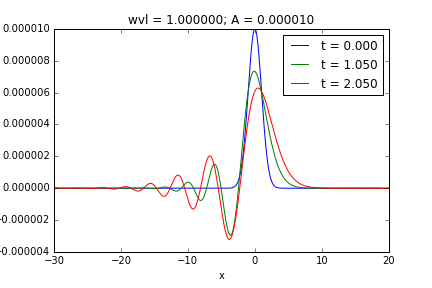
\includegraphics[scale=.45]{figures/criteria6.png}
		\caption{Short gaussian wave 		\label{fig:KdVcriteriaShort}}
	\end{subfigure}
	\begin{subfigure}{.5\linewidth}
		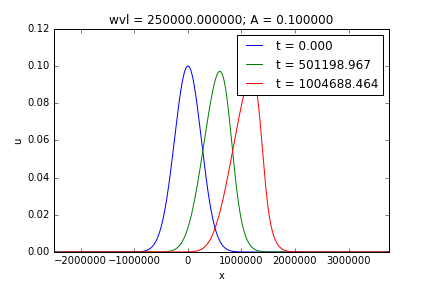
\includegraphics[scale=.45]{figures/criteria5.png}
		\caption{Long gaussian wave		\label{fig:KdVcriteriaLong}}
	\end{subfigure}
	\caption{Simulations with the KdV equation 	\label{fig:KdVcriteria}}
\end{figure}

\paragraph{Conclusions :}

\begin{itemize}
 \item These results are compatible with the observations and examples made by \cite{conservationLaws2002}, which states that dispersive effects are stronger in shorter waves; in the long wave, the nonlinear effect is more evident.
 \item The range of validity of the KdV equation is very small in the case of the short wave, and much larger for the long wave. This is coherent with the fact that this model is a good approximation for the propagation of long waves with small finite amplitude, which can be seen in the definition of $h_0^{valid}$ (equation \eqref{eq:hvalid}) : reducing $A$ and increasing $\lambda$ increases the length of the interval of validity.
 \item One of our conclusions in the derivation of the proposed criteria should be revised : the one which says that the importance of the dispersive over the nonlinear effects can be measured by $\alpha^2 = \frac{h_0^2}{6}$ : in fact, in the given examples, if we adopt $h_0$ as the median of $ h_0^{valid} $, the highly-dispersive short wave has a smaller $\alpha^2$ than the long wave.
\end{itemize} 
\section{BBM equation}
\label{sec:BBM}

\subsection{The model}

\indent The second model for wave propagation that we consider in this project is the BBM equation, which models a long-wave propagation accounting for nonlinear and dispersive effects (in an alternative formulation for the KdV equation, with better stability and numerical properties). This equation is derived by \ref{BBM1971} and reads

\begin{equation}
    u_t + u_x + (u^2)_x - u_{xxt} = 0 \ , \ \ x \in [x_{min},x_{max}], \ \ t \in [0, t_{max}] \\
\end{equation}

\subsection{Discretization}

\indent The BBM model will be treated here in the same way we did for the KdV equation : we will use an split method, leading to the resolution of the following problem in each time step: 

\begin{equation}
\begin{cases}
    v_t + v_x + (v^2)_x = 0 \ \ ,\ t \in [t_n,t_{n+1}], \  v(t_n) = u(t_n) \\
    w_t - cw_{xxt} = 0 \ \ , \ t \in [t_n,t_{n+1}], \  w(t_n) = v(t_{n+1}) \\
    u(t_{n+1}) = v(t_{n+1})
\end{cases}
\end{equation}

\noindent given an initial solution and appropriate boundary conditions.

\indent The first equation (which is exactly the same as in the KdV equation) will be solved with a Finite Volume method, with a 4th order Runge-Kutta discretization for the time derivative, as described in the section \ref{sec:KdVSplitted1}.  The second equation will be solved with a Fourier spectral method in the periodic case, and a finite difference method in the nonperiodic one, as described below :

\paragraph{Periodic case}

\indent The second equation of the BBM splitted model can be written as

$$(w - cw_{xx})_t=0$$

\noindent showing that $w - w_{xx}$ does not depend on time. Therefore, for each time step $[t_n,t_{n+1}] : $

$$w - cw_{xx} = (w - cw_{xx})\rvert_{t=t_n} = (v - cv_{xx})\rvert_{t=t_{n+1}} = g(x)$$

\indent This equation will be solved using the Fourier method. Let $\hat{w}(k,t_n)$ and $\hat{g}(k)$ be the Fourier coefficients of $w(x,t_n)$ and $g(x)$ respectively.  The Fourier transform of the above equation gives

$$(\hat{w})(k,t) = \frac{\hat{g}(k)}{1+ck^2}$$

\indent The right-hand side of the last equation does not depend on time. Therefore, the inverse Fourier transform using the coefficients $\hat{w}(k,t)$ gives $w(x,t_{n+1})$

\paragraph{Nonperiodic case}

...

\subsection{Simulations}

...
\section{Serre equation}
\label{sec:Serre}

\subsection{The model}

\indent The Serre equations are a model to describe highly nonlinear waves propagating in shallow waters. Considering a horizontal bottom, these equations are written as

\begin{equation}
\label{eq:SerreFull}
h_t + (hu)_x = 0 \\
u_t + uu_x + gh_x - \frac{1}{3h}\left(h^3 \left( u_{xt} + uu_{xx} - (u_x)^2  \right) \right)_x = 0
\end{equation}

\noindent where $u = u(x,t)$, $h = h(x,t)$ and $g$ are, respectively, the depth-averaged horizontal velocity of the fluid, the water depth and the gravity acceleration. This formulation is based on \cite{CarterCienfuegos2011}.

\subsection{Discretization}

\indent As done previously for the numerical resolution of the KdV and the BBM equations, the Serre equations will be numerically solved using a splitting method, in which the system of equations will be decomposed in two : the first one will contain the advection terms, and the second one, all the high-order derivative terms.

\indent Therefore, the numerical resolution will consist in solve, in each time step $[t_n, t_{n+1}]$, the following problem :

\begin{equation}
\label{eq:SerreSplit1}
\begin{cases}
\th_t + \left(\th\tu\right)_x = 0 \\
\tu_t + \tu\tu_x + g\th_x = 0, \ \, t \in [t_n, t_{n+1}], \ \  (\th,\tu)(x,t_n) = (h,u)(x,t_n)
\end{cases}
\end{equation}

\begin{equation}
\label{eq:SerreSplit2}
\begin{cases}
\lh_t   = 0 \\
\lu_t - \frac{1}{3\lh}\left(\lh^3 \left( \lu_{xt} + \lu\lu_{xx} - (\lu_x)^2  \right) \right)_x = 0, \ \, t \in [t_n, t_{n+1}], \ \  (\lh,\lu)(x,t_n) = (\th,\tu)(x,t_{n+1})
\end{cases}
\end{equation}

\begin{equation}
\begin{cases}
(h,u)(x,t_{n+1}) = (\lh,\lu)(x,t_{n+1})
\end{cases}
\end{equation}

\indent If we denote the two systems by the operators $T_a^{\Delta t}$ and $T_d^{\Delta t}$, respectively, where the superscript indicates that the operator is performed over a time step $\Delta t$, the problem can be written as

\begin{equation}
(h,u)(x,t_{n+1}) = T_d^{\Delta t} \left( T_a^{\Delta t} \left((h,u)(x,t_n) \right) \right)
\end{equation}

\indent Some variations of the splitting scheme were also implemented. For example, inverting the order of the operators; or the method known as "Strang splitting", in which three problems are solved in each time-step :

\begin{equation}
(h,u)(x,t_{n+1}) = T_a^{\frac{\Delta t}{2}} \left( T_d^{\Delta t} \left( T_a^{\frac{\Delta t}{2}} (h,u)(x,t_n) \right) \right)
\end{equation}

\noindent In the following descriptions of the resolution of the two schemes, the tilde and the overbar will be omitted for the sake of clarity.

\subsubsection{First system of equations (advection step)}

\noindent The first part of the Serre equation corresponds to the Non linear Shallow Water equation, that after noticing that 

\begin{align*}
(hu)_t &= uh_t + hu_t = -u(hu)_x - h\left(uu_x + gh_x\right) \\
	&= -u\left (h_xu + 2hu_x \right) - ghh_x  \\
	&= -\left(hu^2\right)_x - \frac{1}{2}g\left(h^2\right)_x = - \left(hu^2 +  \frac{1}{2}gh^2 \right)_x
\end{align*}
\noindent it can be written as a conervation law of the form

\begin{equation}
	U_t + F(U)_x = 0
	\label{serre:conservative_swe}
\end{equation}

\noindent where $U=(h,hu)^T$, $F(U) = (hu, hu^2 + \frac{1}{2}gh^2)$. Weak solutions are approximated using a Finite Volume scheme, that is, after integrating the system \eqref{serre:conservative_swe} in a cell $\Omega_i = [x_i-\Delta x/2, x_i+\Delta x/2]$, and defining $ \overline U = \frac{1}{\Delta x} \int_{\Omega_i} U(x)dx$, then the semidiscrete approximation to \eqref{serre:conservative_swe} is 

\begin{equation}
	\overline U _t + \frac{1}{\Delta x}\left( F(U_{i+1/2}) - F(U_{i-1/2}) \right) = 0
\end{equation}

\noindent where $U_{i\pm1/2}$ corresponds to the values of the conserved variables at the interface of each cell. 

The values at each interface $U^* = U_{i+1/2}$ are obtained from the solution to the Riemann problem of the non-conservative form of \eqref{serre:conservative_swe} between two states $U_L = U_i$ and $U_R = U_{i+1}$

\begin{equation}
	\begin{split}
	  U_t + A(U) U_x = 0 \\
	  U(t=0,x) = \begin{cases}
		 U_l &, \text{ if } x\leq 0. \\
		 U_r &, \text{ if } x > 0 
		\end{cases}
	\end{split}
	\label{serre:nonconservative_swe_1}
\end{equation}

\noindent where $A$ is the jacobian matrix of $F(U)$. The solution to this Riemann problem is found using the approximate Riemann solver of Roe that is described in reference \cite{marche2006}. It consists first of a change of variables that allows to write \eqref{serre:nonconservative_swe_1} as

\begin{equation}
	\begin{split}
	  V_t + C(V)V_x = 0 \\
	  V(t=0,x) = \begin{cases}
		V_l &, \text{ if } x\leq 0. \\
	 V_r &, \text{ if } x > 0 
		\end{cases}
	\end{split}
	\label{serre:nonconservative_swe_2}
\end{equation}

\noindent with $V = (2c,u)^T$ and 
$C(V) = \left( 
\begin{array}{cc} 
u & c \\ 
c & u \end{array}\right)$. Second, instead of using the exact formulation, a linearized problem is solved using $C(\hat V)$ in place of $C(V)$, with $\hat V = (V_L +V_R)/2$. The matrix $C(\hat V)$ is diagonalizable and thus, a decoupled system can be obtained in the form

\begin{equation}
	\begin{split}
		(w_1)_t + \hat \lambda_1 (w_1)_x = 0\\
		(w_2)_t + \hat \lambda_2 (w_2)_x = 0 \\	
	(w_1,w_2)^T(t=0,x) = \begin{cases}
		((w_1)_L,(w_2)_L)^T &, \text{ if } x\leq 0. \\
		((w_1)_L,(w_2)_L)^T &, \text{ if } x > 0 
		\end{cases}
	\end{split}
\end{equation}

\noindent where $\hat \lambda_1 = \hat u - \hat c$, $\hat \lambda_2 = \hat u + \hat c$, $w_1 = u-2c$, $w_2 = u+2c$ and $ (w_1)_L = u_L - 2c_L, (w_2)_L = u_L - 2c_L$, $ (w_1)_R = u_R - 2c_R, (w_2)_R = u_R - 2c_R$. Writing $W=(w_1,w_2)$ and using index $*,L,R,$ for the values at the interface, left and right states, and noticing that $\hat \lambda_1 \leq \hat \lambda_2$, the solution can be found for separate cases:

\begin{itemize}
	\item If $\lambda_1 > 0$, then $W^* = W_L$
	\item If $\lambda_1 \leq 0 $ and $\lambda_2>0$, $W^* = ((w_R)_1, (w_L)_2)^T$
	\item If $\lambda_2\leq 0 $, $W^* = W_R$
\end{itemize}

\noindent the values at the interface can then be recovered setting the inverse transformation 

\begin{equation}
	u^* = \frac{1}{2}(w^*_1+w^*_2) \\
	h^* = \frac{1}{16g}(w^*_2-w^*_1)^2
	\label{serre:riemman_solution}
\end{equation}

A third step is necessary, which consists on an entropy fix to select only weak solutions that are physically consistent. This is simply obtained by setting $W^* = \hat W$ whenever $(\lambda_1)_L < 0$ and $(\lambda_1)_r >0$, or $(\lambda_2)_L < 0 $ and $(\lambda_2)_R>0$.

\paragraph{Second order Finite Volume Scheme}

To obtain second order convergence for smooth solutions a MUSCL (Monotonic Upstream-Centered Scheme) is used. This means that instead of solving a Riemann problem between $U_L=U_{i}$ and $U_R=U_{i+1}$ one must solve for $U_L = U_{i+1/2^-}$ and $U_{i+1/2^+}$, where $U_{i+1/2^+} = U_i + \frac{\Delta x}{2} s$,  $s = minmod(s_L,s_R)$, 
$s_L = \frac{U_{i}-U_{i-1}}{\Delta x}$, 
$s_R = \frac{U_{i+1}-U_{i}}{\Delta x}$ and

\begin{equation}
	minmod(s_1,s_2) = \begin{cases}
		min(s_1,s_2) & \text{ if } s_1>0 \textit{ and } s_2>0 \\
		max(s_1,s_2) & \text{ if } s_1<0 \textit{ and } s_2<0 \\
		0 & elsewhere
	\end{cases}
\end{equation}

\subsubsection{First system of equations (advection step)}

\indent In the second system (\ref{eq:SerreSplit2}) of the splitted Serre equations , the water depth $h$ is constant in time, and therefore only the velocity $u$ must be updated. Separating the terms containing time derivatives, the second equation of thi system can be rewritten as

\begin{equation}
\label{eq:dispersive}
\left( u - hh_xu_x - \frac{1}{3}h^2u_{xx} \right)_t  - \frac{1}{3h}\left(h^3 \left( uu_{xx} - (u_x)^2  \right) \right)_x = 0
\end{equation}

\indent This equation will be solved using an explicit Finite Difference scheme. Defining

$$g_1 = h^3 \left( uu_{xx} - (u_x)^2 \right)$$

$$g_2 = u - h h_x u_x - \frac{1}{3}h^2 u_{xx}$$

\noindent where the derivatives are evalueated using appropriate finite difference approximations.

\indent With this notation, using an one-step forward time discretization, one gets

$$(g_2)_i^{n+1} = (g_2)_i^n + \frac{\Delta t}{3h_i^n} \left(\left( g_1 \right)_x\right)_i^n = G_i^n$$

\noindent where the superscript and the subscript denotes respectively the time step and the spatial position.

\indent Using 2nd order centered approximation for the spatial derivatives in $(g_2)_i^{n+1}$, one gets the following tridiagonal linear system :

$$\left( \frac{h_i^n(h_x)_i^n}{2\Delta x} - \frac{(h_i^n)^2}{3\Delta x^2} \right)u_{i-1}^{n+1} + 
 \left( 1 + \frac{2(h_i^n)^2}{3\Delta x^2} \right)u_{i}^{n+1} + 
 \left( -\frac{h_i^n(h_x)_i^n}{2\Delta x} - \frac{(h_i^n)^2}{3\Delta x^2} \right)u_{i+1}^{n+1} = G_i^n $$
 
\noindent with the appropriate modifications to take in account the boundary conditions.
 
 
\paragraph{Alternative resolution of the second system (for the variables $(h,hu)$)}
 
\indent Inspired by the discretization described in \cite{Bonneton2011}, we will rewrite the second system of equations obtained in the splitting of the Serre equations, in order to solve it in the variables $(h,hu)$ and thus keep the formulation of the first system.
 
\indent For this purpose, we will multiply the equation (\ref{eq:dispersive}) and write the variable $u$ inside the time derivative as $\frac{1}{h} hu$ :
 
 \begin{equation}
\label{eq:dispersive2}
\left( hu - h^2h_x \left( \frac{1}{h} hu \right)_x - \frac{1}{3}h^3\left( \frac{1}{h} hu \right)_{xx} \right)_t  - \frac{1}{3}\left(g_1 \right)_x = 0
\end{equation}

\indent Developing the spatial derivatives in (\ref{eq:dispersive2}), we get

\begin{equation}
\label{eq:dispersive3}
       \left( 1-h^2 - \frac{h^3}{h_{xx}} \right)(hu) + \left( -hh_x - \frac{2h^3}{3h_{x}} \right)(hu)_x + \left( - \frac{h^2}{3} \right)(hu)_{xx} - \frac{1}{3}\left(g_1 \right)_x = 0
\end{equation}

\noindent which can be written as

\begin{equation}
    \tilde{T} (hu)_t = \frac{1}{3}\left(g_1 \right)_x \rightarrow (hu)_t = \tilde{T}^{-1}\left(\frac{1}{3}\left(g_1 \right)_x\right)
\end{equation}

\noindent where $\tilde{T} = 1 + hT\frac{1}{h} $

\noindent and $T$ is an operator defined by Bonneton et al and given by (in the 1D case)

\begin{equation}
   Tw = -\frac{h^2}{3}w_{xx} - hh_xw_x
\end{equation}

\indent Therefore, for each $i=1,...N-1$, the actualization of the solution in time is given by

\begin{equation}
(hu)_i^{n+1} = (hu)_i^n + \Delta t z_i^n
\end{equation}

\noindent where $Z = (z_1,z_2,...,z_{n+1})^T$ is solution of $\tilde{T}Z = \frac{1}{3}\left(g_1 \right)_x$. The left side of this system has the form

\begin{equation}
h\frac{z}{h} - h^2h_x \left( \frac{z}{h} \right)_x - \frac{1}{3}h^3\left( \frac{z}{h}\right)_{xx}
\end{equation}

\noindent which is solved in the variable $z/h$ (in order to avoid divisions by spatial derivatives of $h$, that can be equal to zero), leading to the 2nd order discretization

\begin{equation}
\begin{split}
\left( \frac{h_i^n(h_x)_i^n}{2\Delta x} - \frac{(h_i^n)^2}{3\Delta x^2} \right)  \left( \frac{z}{h} \right)_{i-1}^{n+1} + 
 \left( 1 + \frac{2(h_i^n)^2}{3\Delta x^2} \right)\left( \frac{z}{h} \right)_{i}^{n+1} + \\
  \left( -\frac{h_i^n(h_x)_i^n}{2\Delta x} - \frac{(h_i^n)^2}{3\Delta x^2} \right)\left( \frac{z}{h} \right)_{i+1}^{n+1} = \frac{1}{3} \left(\left( g_1 \right)_x\right)_i^n
  \end{split}
\end{equation}

\subsection{Simulations}

\subsubsection{Description of the initial solution}

\indent In order to validate the implementation of the Serre equations, we will solve it using as initial solution the analytical solution. According to \cite{CarterCienfuegos2011}, the Serre equations admit the following family of periodic solutions

\begin{align*}
    h(x,t) &= a_0 + a_1 dn^2(\kappa(x-ct),k) \\
    u(x,t) &= c\left( 1 - \frac{h_0}{h(x,t)}\right)
\end{align*}

\begin{align*}
    \kappa &= \frac{\sqrt{3a_1}}{2\sqrt{a_0(a_0+a_1)(a_0+(1-k^2)a_1)}} \\
    c &= \frac{\sqrt{g a_0(a_0+a_1)(a_0+(1-k^2)a_1)}}{h_0}
\end{align*}

\noindent with $k\in(0,1)$, $a_0>0$ and $a_1>0$, $dn(\cdot,k)$ is a Jacobi elliptic function with elliptic modulus $k$.

\indent The relation between the wavelength $\lambda$ and $k\in(0,1)$ is $$\lambda = \frac{2K(k)}{\kappa}$$ and the mean water depth, $h_0$ is computed as $$h_0 = \frac{1}{\lambda}\int_{0}^\lambda h(x,t)dx = a_0 + a_1 \frac{E(k)}{K(k)}$$

\noindent with $K(k)$ and $E(k)$ are the complete elliptic integrals of the first and second kinds.

\indent The limit for $k\to0^+$ is constant water level $a_0+a_1$ at rest. If $k\to1^-$ it converges to the Rayleigh solitary wave solution. We will also test this last case, in which the solution is described by

\begin{align*}
    h(x,t) &= a_0 + a_1 sech^2(\kappa(x-ct),k) \\
    u(x,t) &= c\left( 1 - \frac{a_0}{h(x,t)}\right)
\end{align*}

\begin{align*}
    \kappa &= \frac{\sqrt{3a_1}}{2\sqrt{a_0(a_0+a_1)}} \\
    c &= \sqrt{g a_0(a_0+a_1)}
\end{align*}

\indent The expressions for the wavelength $\lambda$ and the mean water depth $h_0$ are the same as shown for the general case of the cnoidal solution.

\subsubsection{Results}

\indent With the objective to observe the nonlinear and the dispersive processes in the model, we solved the Serre equation and the Nonlinear Shallow Water Equation (NSWE), which is the first step of the proposed split scheme. The figures \ref{fig:cnoidalh} and \ref{fig:cnoidalu} shows the evolution of $(h,u)$ for the cnoidal solution; and the figures \ref{fig:solitaryh} and \ref{fig:solitaryu} for the solitary solution. In this last case, we also solved the problem with a first order finite volume solver for the resolution of the first step of the Serre equation.

\begin{figure}[h!]
	\begin{subfigure}{.3\linewidth}
		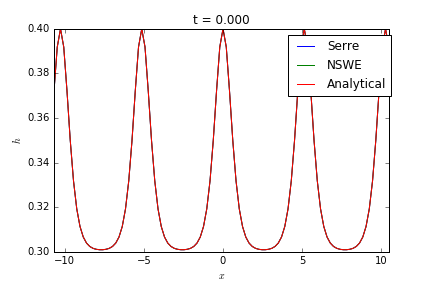
\includegraphics[scale=.3]{figures/Serre/cnoidal1h.png}	
	\end{subfigure}
	\begin{subfigure}{.3\linewidth}
		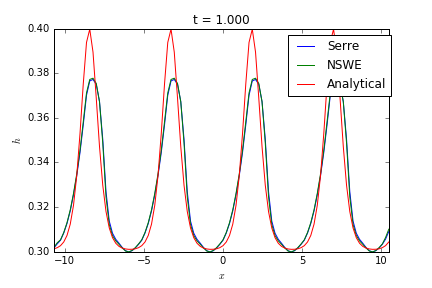
\includegraphics[scale=.3]{figures/Serre/cnoidal2h.png}	
	\end{subfigure}
	\begin{subfigure}{.3\linewidth}
		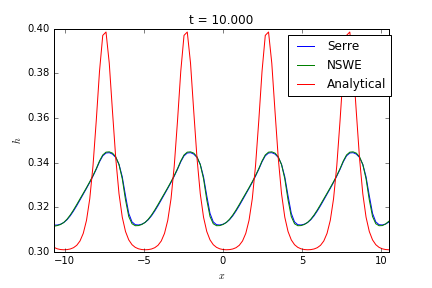
\includegraphics[scale=.3]{figures/Serre/cnoidal3h.png}	
	\end{subfigure}
	\caption{Evolution of $h$ for the cnoidal solution in the Serre equation \label{fig:cnoidalh}}
\end{figure}

\begin{figure}[h!]
	\begin{subfigure}{.3\linewidth}
		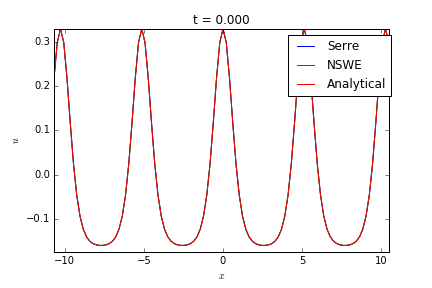
\includegraphics[scale=.3]{figures/Serre/cnoidal1u.png}	
	\end{subfigure}
	\begin{subfigure}{.3\linewidth}
		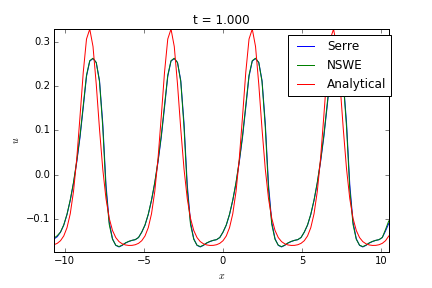
\includegraphics[scale=.3]{figures/Serre/cnoidal2u.png}	
	\end{subfigure}
	\begin{subfigure}{.3\linewidth}
		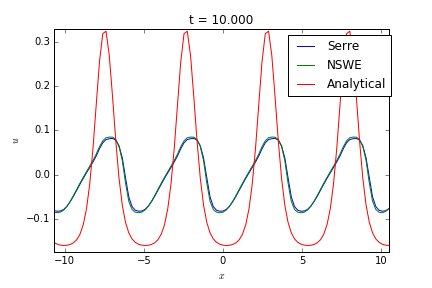
\includegraphics[scale=.3]{figures/Serre/cnoidal3u.png}	
	\end{subfigure}
	\caption{Evolution of $u$ for the cnoidal solution in the Serre equation \label{fig:cnoidalu}}
\end{figure}

\begin{figure}[h!]
	\begin{subfigure}{.3\linewidth}
		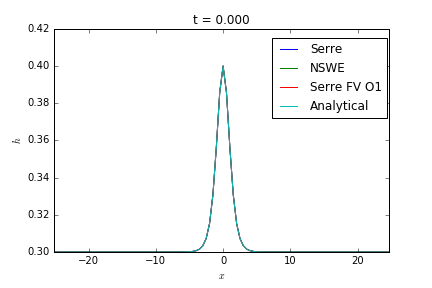
\includegraphics[scale=.3]{figures/Serre/solitary1h.png}	
	\end{subfigure}
	\begin{subfigure}{.3\linewidth}
		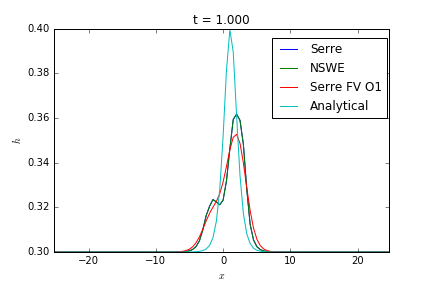
\includegraphics[scale=.3]{figures/Serre/solitary2h.png}	
	\end{subfigure}
	\begin{subfigure}{.3\linewidth}
		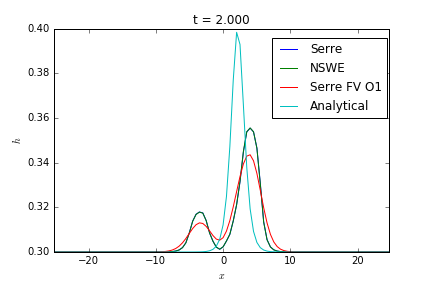
\includegraphics[scale=.3]{figures/Serre/solitary3h.png}	
	\end{subfigure}
	\caption{Evolution of $h$ for the solitary solution in the Serre equation \label{fig:solitaryh}}
\end{figure}

\begin{figure}[h!]
	\begin{subfigure}{.3\linewidth}
		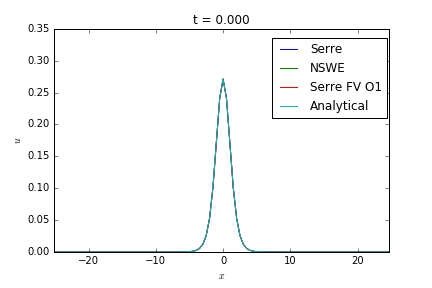
\includegraphics[scale=.3]{figures/Serre/solitary1u.png}	
	\end{subfigure}
	\begin{subfigure}{.3\linewidth}
		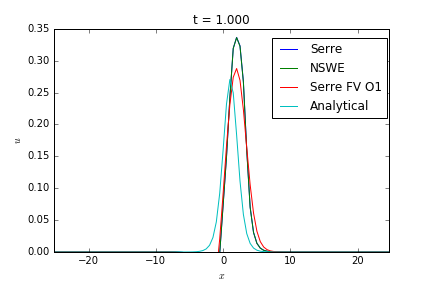
\includegraphics[scale=.3]{figures/Serre/solitary2u.png}	
	\end{subfigure}
	\begin{subfigure}{.3\linewidth}
		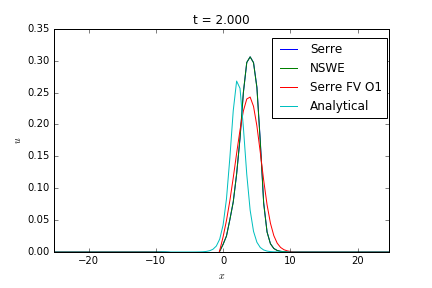
\includegraphics[scale=.3]{figures/Serre/solitary3u.png}	
	\end{subfigure}
	\caption{Evolution of $u$ for the solitary solution in the Serre equation \label{fig:solitaryu}}
\end{figure}

\indent The results show the existence of modeling or programming errors. In both cases tested, the analytical solution is not preserved : we observe a strong dissipation of the solution, and, in the solitary wave case, a inversion of the velocity that causes the formation of secondary waves. The utilization of a higher-order solver for the Finite Volume scheme did not corrected this last problem, but showed a lower dissipation.
\section{Study of transparent boundary conditions}
\label{sec:TBC}

\subsection{Introduction and motivational examples}

\indent The work presented in this section is an introduction to the objectives that we are looking for in this project, concerning the study of Transparent Boundary Conditions (TBCs). It was developed on the KdV equation, because, among the models studied and implement until here (KdV, BBM and Serre equations), it was the one for which we have obtained the best computational implementation.

\indent The TBCs are constructed such that the solution computed in the finite computational domain $\Omega$ coincides with the solution of the whole-space problem, restricted to $\Omega$ . In general, these boundary conditions are nonlocal in time,  so they must be approximated for an efficient numerical implementation \cite{Xavieretal2008}. Before moving to the models of wave propagation, in order to see in practice this definition we will implement a simple example, with analytical solution and TBCs, derived following \cite{Japhet2003}.  We will consider the 1D problem 

\begin{equation}
\begin{cases}
-u''(x) = 1 \ \ in \ \ \Omega = [0,2]\\
u(0) = 0 \\
u(2) = 0
\end{cases}
\end{equation}

\noindent whose solution is

$$u(x) = -\frac{x^2}{2} + x$$

\noindent and, considering the partition of $\Omega$ in $\Omega_1 = [0,1]$ and $\Omega_2 = [1,2]$, we will solve the problem

\begin{equation}
\begin{cases}
-u_1''(x) = 1 \ \ in \ \ \Omega_1\\
u_1(0) = 0 \\
B(u_1) = 0 \ \ at \ \ \Gamma=\{1\}
\end{cases}
\end{equation}

\noindent where the transparent boundary condition $B(u)$ is such that $u|_{\Omega_1} = u_1$.

\indent The TBC is written in the form $B(u) = \frac{\partial}{\partial x}u + D2N(u)$, where the D2N (Dirichlet to Neumann) operator is defined by

$$\left. D2N : \alpha(x) \mapsto \frac{\partial}{\partial x}v \right\rvert_\Gamma$$

\noindent where $\alpha$ is defined in the boundary $\Gamma$. In the case treated here, $\Gamma$ is a point, and therefore $\alpha$ is a scalar.

\indent The function $v$ is solution of

\begin{equation}
\begin{cases}
-v''(x) = 1 \ \ in \ \ \Omega_2\\
v(2) = 0 \\
v(1) = \alpha \ \ at \ \ \Gamma=\{1\}
\end{cases}
\end{equation}

\noindent so

$$v(x) = -\frac{x^2}{2} + \left(\frac{3}{2} - \alpha \right) + 2\alpha -1$$

\noindent and 

$$\left. \frac{\partial}{\partial x}v \right\rvert_{x=1} = \frac{1}{2} - \alpha$$

\indent Finally, the TBC reads

$$B(u_1) = \frac{\partial}{\partial x}u_1 + D2N(u_1) = \frac{\partial}{\partial x}u_1+ \frac{1}{2} - u_1$$

\indent The problem was solved with a finite difference method, with centered second-order approximation for the spatial derivative, for two different grids. The figure \ref{fig:TBClaplace} shows that the constructed TBC effectively provides a convergent solution.

\begin{center}
	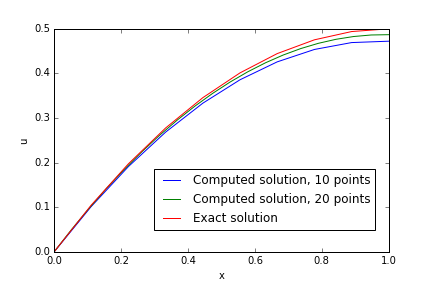
\includegraphics[scale=.5]{figures/TBClaplace.png}
	\captionof{figure}{Solutions for the Laplace equation with TBC \label{fig:TBClaplace}}
\end{center}

\indent Coming back to the wave models, we recall that, in the first simulations with the splitting method adopted to the resolution of the KdV equation, we did not make a rigorous application of appropriate boundary conditions. In fact, our initial objective was to validate the method; therefore, imposing periodic or homogeneous Dirichlet and Neumann conditions, we analyzed the evolution of the solution only before the arrival of the wave to the boundaries.

\indent The following example shows very clearly the influence of inappropriate boundary conditions on the solution. We solved two times the same problem, with the same initial solution, boundary conditions, and spatial and time discretizations: 

\begin{equation}
    \begin{cases}
    u_t + u_x + (u^2)_x + u_{xxx} = 0 \ , \ \ x \in \Omega=[a,b] \ \ t \in [0, t_{max}] \\
    u(x,0) = \Phi(x) \\
    u(a,t) = 0 \\
    u(b,t) = 0 \\
    u_x(b,t) = 0  \\ 
    \end{cases}
\end{equation}

\indent The only difference is the size of the domain of each problem : they were chosen such that the wave reaches the boundaries (within the maximal time of simulation) in the first problem, but not in the second. The difference between the solution increases with the time, beginning in the boundary and propagating to the whole domain :

\begin{figure}[h]
	\begin{subfigure}{.3\linewidth}
		\center
		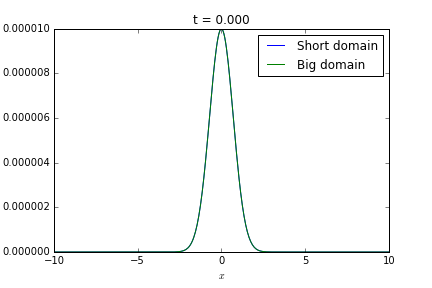
\includegraphics[scale=.3]{figures/motivational1A.png}	
	\end{subfigure}
	\begin{subfigure}{.3\linewidth}
		\center
		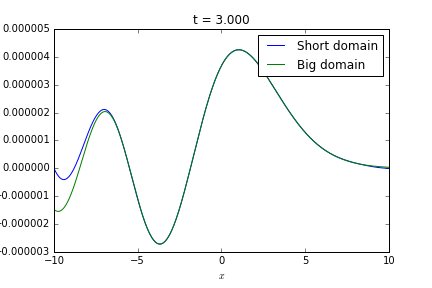
\includegraphics[scale=.3]{figures/motivational1B.png}	
	\end{subfigure}
	\begin{subfigure}{.3\linewidth}
		\center
		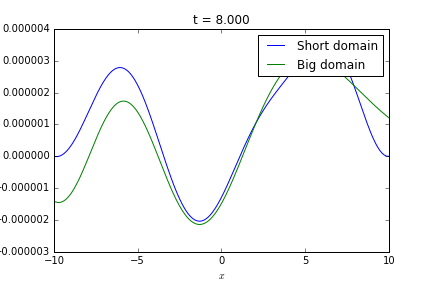
\includegraphics[scale=.3]{figures/motivational1C.png}	
	\end{subfigure}
	\caption{First motivational example : comparison between the solutions in a small and a big domain}
\end{figure}

\indent Therefore, we look for boundaries conditions that can efficiently simulate the called Transparent Boundary Conditions (TBCs), i.e., in a such a way that the solution calculated in the computational domain $\Omega$ coincides with solution of the whole-space restricted to $\Omega$. As a consequence, we want the boundaries not to have an influence on the solution, so, when the wave reaches the boundary, it will simply "exit" the domain. The following example shows another motivation for this work.

\indent We want to solve the following problem :

\begin{equation}
    (P_1) \begin{cases}
    u_t + u_x + (u^2)_x + u_{xxx} = 0 \ , \ \ x \in \Omega_1 = [0,L], \ \ t \in [0, t_{max}] \\
    u(x,0) = \Phi(x) \\
    u(0,t) = 0 \\
    u_x(0,t) = 0 \\
    u(L,t) = g(t)  \\ 
    \end{cases}
\end{equation}

\indent We seek a function $g(t)$ to simulate the TBC. In order to do this, we will solve before the problem

\begin{equation}
    (P_2) \begin{cases}
    u_t + u_x + (u^2)_x + u_{xxx} = 0 \ , \ \ x \in \Omega_2 = [0,2L], \ \ t \in [0, t_{max}] \\
    u(x,0) = \Phi(x) \\
    u(0,t) = 0 \\
    u_x(0,t) = 0 \\
    u(2L,t) = 0  \\ 
    \end{cases}
\end{equation}

\noindent and we impose $g(t) = u_2(t)$, where $u_2$ is the solution of $(P_2)$. To obtain more precise results, the two computations are made with the same mesh size and time step.

\indent Suppose that there is a unique solution $u_1$ to $(P_1)$. We can easily see that $u_2|_{\Omega_1}$ is also a solution of $(P_1)$. Therefore, $u_1 = u_2|_{\Omega_1}$. It justifies why our procedure works as a TBC, as shown in the figure \ref{fig:motivation2} (close-up in the region close to the right boundary) :

\begin{figure}[h]
	\begin{subfigure}{.5\linewidth}
		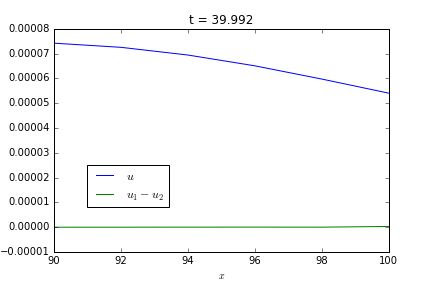
\includegraphics[scale=.5]{figures/motivational2A.png}	
	\end{subfigure}
	\begin{subfigure}{.5\linewidth}
		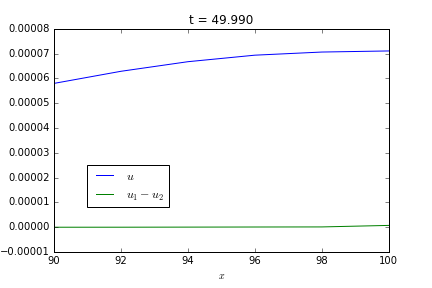
\includegraphics[scale=.5]{figures/motivational2B.png}	
	\end{subfigure}
	\caption{Second motivational example : solution with an "exact" Dirichlet condition at the right boundary \label{fig:motivation2}}
\end{figure}

\subsection{Optimization of Robin boundary conditions to simulate TBCs}

\subsubsection{Robin boundary conditions up to the first derivative}

\indent Although the motivating result presented in the above example, we cannot apply this procedure in practice. In fact, computing the solution in a larger domain and using it as exact solution is only a trick, which has no practical interest. Therefore, we want to determinate approximations for a TBC without having a referential solution. 

\indent The KdV will be solved in the domain $[-L,L]$ with the following boundary conditions (imposed in the resolution of the second equation of the split method):

\begin{equation}
\begin{cases}
    u(-L) = 0 \\
    u_x(-L) = 0 \\
    \alpha u(L) + \beta u_x(L) = 0,  \ \ \alpha,\beta > 0
\end{cases}
\end{equation}

\indent In the third condition, called a Robin boundary condition, the parameters $\alpha$ and $\beta$ (or, equivalently, the parameter $\beta/\alpha$) will be optimized in order to simulate a TBC. In a first moment, we will consider Robin BCs up to the first derivative of the solution.

\indent To find the optimal coefficients, we will test several pairs $(1,\beta/\alpha)$ (including the limits $\beta/\alpha \rightarrow 0$ and $\beta/\alpha \rightarrow \infty$, corresponding respectively to Dirichlet and Neumann BCs) and compute the error regarding to a referential solution $u_{ref}$, computed in a domain $[-2L,2L]$. Two errors will be computed, for each time step $t_n$ :

\begin{equation}
e_1^n = \sqrt{\sum_{i=0}^N{\left( u^n_i - (u_{ref})^n_i\right)^2}} 
\end{equation}

\begin{equation}
e_2^n =  u^n_N - (u_{ref})^n_N
\end{equation}

\indent $e_2^n$ is computed in order to show that most part of the error $e_1^n$ of the entire domain occurs in the boundary.

\indent The figures \ref{fig:robin1} to \ref{fig:robinErrorsExample} show some snapshots and the evolution of $e_1$ and $e_2$ for some values of $\beta/\alpha$ . The figure \ref{fig:robinErrorsAll} compares $e_2$ for many other values, including the pure Dirichlet (with $\alpha = 1, \beta = 0$, so $log(\beta/\alpha) = -\infty$) and pure Neumann (with $\alpha = 0, \beta = 1$)  conditions.


\begin{figure}[h]
	\begin{subfigure}{.5\linewidth}
		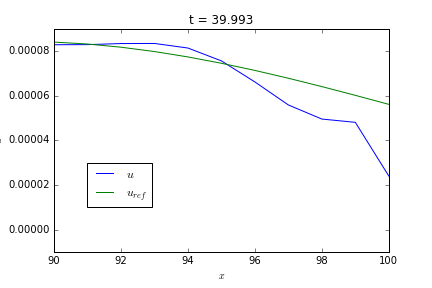
\includegraphics[scale=.5]{figures/robin1A.png}	
	\end{subfigure}
	\begin{subfigure}{.5\linewidth}
		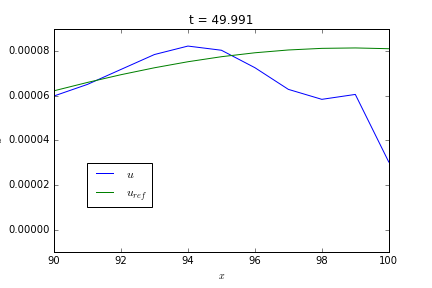
\includegraphics[scale=.5]{figures/robin1B.png}	
	\end{subfigure}
	\caption{Computed and the referential solution for  $\beta/\alpha = 1$ \label{fig:robin1}}
\end{figure}

\noindent\begin{minipage}{\textwidth} 
	\begin{minipage}{.5\textwidth} 
		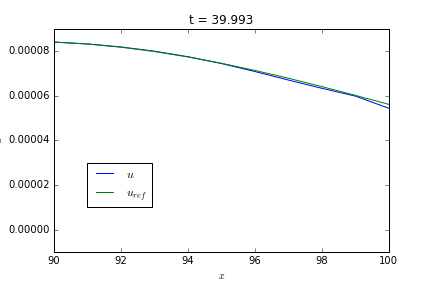
\includegraphics[scale=.5]{figures/robin10A.png}	
	\end{minipage}
	\begin{minipage}{.5\linewidth}
		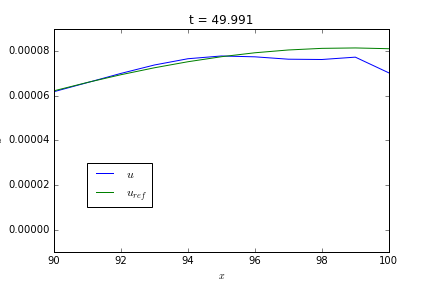
\includegraphics[scale=.5]{figures/robin10B.png}	
	\end{minipage}
	\captionof{figure}{Computed and the referential solution for  $\beta/\alpha = 10$ \label{fig:robin10}}
\end{minipage}

\noindent\begin{minipage}{\textwidth} 
	\begin{minipage}{.5\textwidth} 
		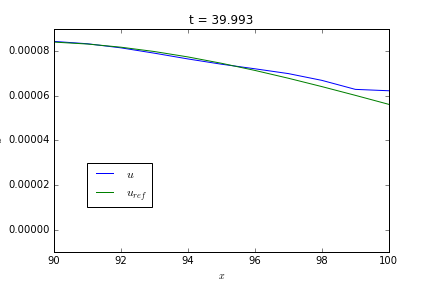
\includegraphics[scale=.5]{figures/robin100A.png}	
	\end{minipage}
	\begin{minipage}{.5\linewidth}
		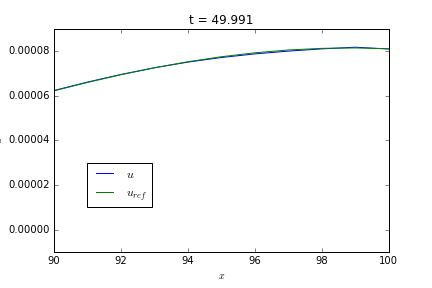
\includegraphics[scale=.5]{figures/robin100B.png}	
	\end{minipage}
	\captionof{figure}{Computed and the referential solution for  $\beta/\alpha = 100$ \label{fig:robin100}}
\end{minipage}

\noindent\begin{minipage}{\textwidth} 
	\begin{minipage}{.3\textwidth} 
		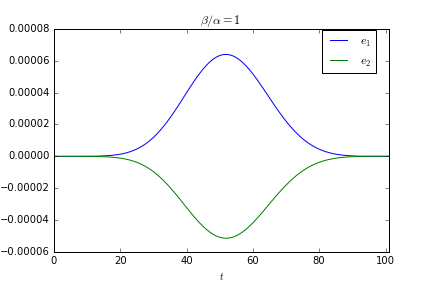
\includegraphics[scale=.3]{figures/robin1Error.png}	
		\captionof{subfigure}{$\beta/\alpha = 1$}
	\end{minipage}
	\begin{minipage}{.3\textwidth} 
		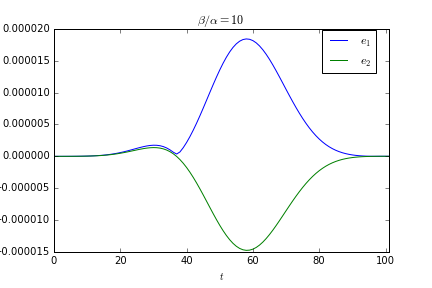
\includegraphics[scale=.3]{figures/robin10Error.png}	
		\captionof{subfigure}{$\beta/\alpha = 10$}
	\end{minipage}
	\begin{minipage}{.3\textwidth}
		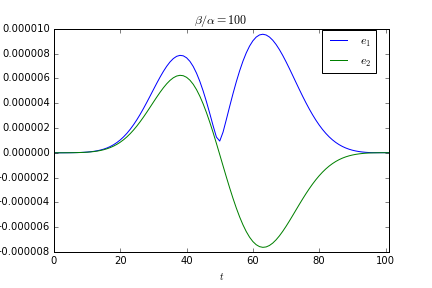
\includegraphics[scale=.3]{figures/robin100Error.png}	
		\captionof{subfigure}{$\beta/\alpha = 100$}
	\end{minipage}
	\captionof{figure}{Errors between the computed and the referential solution \label{fig:robinErrorsExample}}
\end{minipage}

\begin{center}
		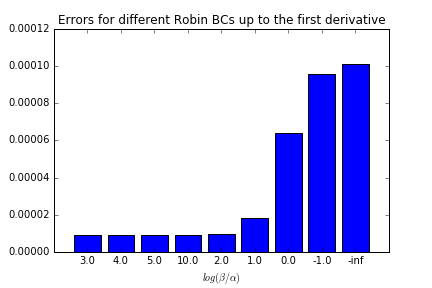
\includegraphics[scale=.6]{figures/robinErrors1.png}
	     \captionof{figure}{Error $||e_1| = \sum_{n=0}^{n_{max}}(e^n_1)^2$ between the computed and the referential solution for many values of $\beta/\alpha$ \label{fig:robinErrorsAll}}
\end{center}


\indent The results presented in the figures \ref{fig:robin1} to \ref{fig:robinErrorsAll} show that boundary conditions with stronger Neumann character produce better approximations to the TBC, compared to more Dirichlet-type conditions. The results for pure Neumann conditions and for Neumann with a small but non-zero Dirichlet were very close, as presented in the table \ref{tab:robinErrorsZoom} for a more refined study around the best values of $\beta/\alpha$. In fact, setting the solution to zero in the boundary is a too much strong condition, and the Neumann condition captures in a more satisfactory way the smoothness of the propagating wave.

\begin{center}
		\begin{tabular}{c|c}
			$log(\beta/\alpha)$ & Error ($\times 10^{-6}$) \\
			\hline
			2.5 & 8.93\\
			3.0 & 8.87\\
			3.5 & 8.95\\
			4.0 & 8.98\\
			4.5 & 8.99\\
			5.0 & 8.99\\
			$\infty$ & 8.99	
		\end{tabular}
		\captionof{table}{Error $||e_1| = \sum_{n=0}^{n_{max}}(e^n_1)^2$ for some values of $\beta/alpha$ around the best ones \label{tab:robinErrorsZoom}}
\end{center}

\subsubsection{Robin boundary conditions up to the second derivative}

\indent We repeated the tests described above, but replacing the boundary condition in the right boundary by $\alpha u(L) + \beta u_x(L) + \gamma u_{xx}(L) = 0,  \ \ \alpha,\beta, \gamma > 0$.

\indent The values of $\alpha$ and $\beta$ will be fixed and equal to the ones that gave the minimal error in the previous simulations ($(\alpha,\beta) = (1,1000)$). We will show directly the graph containing the errors for many values of $\gamma/\beta$ (figure \ref{fig:robinErrorsAll2}, which should be compared with the figure \ref{fig:robinErrorsAll}. Similarly to the previous conclusions, we observe a better approximation of the TBCs for stronger values of $\gamma/\beta$ (being the error almost constant above a certain value, as show in the table \ref{tab:robinErrors2Zoom}). In fact, even the worst error in the figure \ref{fig:robinErrorsAll2} ($||e_1|(\gamma/\beta = 0.01) = 8.78 \times 10^{-6}$) is smaller than the best one of the table \ref{tab:robinErrorsZoom}.

\begin{center}
		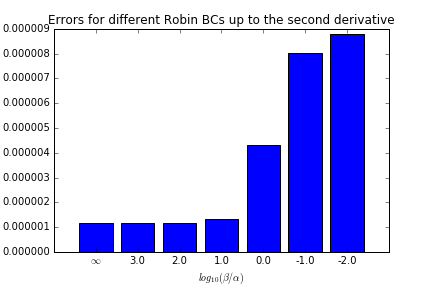
\includegraphics[scale=.6]{figures/robinErrors2.png}
	     \captionof{figure}{Error $||e_1| = \sum_{n=0}^{n_{max}}(e^n_1)^2$between the computed and the referential solution for many values of $\gamma/\beta$, with Robin conditions up to the second derivative \label{fig:robinErrorsAll2}}
\end{center}

\begin{center}
		\begin{tabular}{c|c}
			$log(\gamma/\beta)$ & Error ($\times 10^{-6}$) \\
			\hline
			2.0 & 1.157665\\
			2.5 & 1.157382\\
			3.0 & 1.157280\\
			3.5 & 1.157247\\
			4.0 & 1.157236\\
			4.5 & 1.157233\\
			$\infty$ & 1.157231	
		\end{tabular}
		\captionof{table}{Error $||e_1| = \sum_{n=0}^{n_{max}}(e^n_1)^2$ for some values of $\gamma/beta$ around the best ones \label{tab:robinErrors2Zoom}}
\end{center}

\subsubsection{Partial conclusion} 

\indent Resuming this first study of the Transparent Boundary Conditions, we looked for approximating them by Robin boundary conditions, written in a generic way, with modifiable coefficients for each term (the functions and its derivatives). The idea was to test many combinations of coefficients in order to optimize them (comparing the computed solution in $[-L,L]$ with a referential solution computed in $[-2L,2L]$). As described above, Robin conditions taking in account the continuity of the tested function (i.e., with higher coefficients for the derivative terms) produced better results. Therefore, a TBC based on the first derivative was better than one based only on the solution; and a TBC based on the second derivative was even better. Finally, we observed that, in general, the improvement of the solution is neglectable above a certain relation between the coefficients. 
\section{Conclusions and next steps}

\indent Considering the work done until here and presented in this report, we can point out some further steps and problems to be solved for the continuity of the project.

\indent Concerning the study and implementation of the models for wave propagation, we will mainly focus in the Serre equations. Our first objective is to have a reliable code to its resolution, firstly validating it to a periodic analytical solution and after moving to different types boundary conditions. We will therefore debug the numerical implementation and review the modeling. Possible increasing of the order of the schemes used may be necessary. This work is essential for the future study of Transparent Boundary Conditions applied to the Serre equations.

\indent In parallel, we will continue the study of TBCs. We will initially search in the literature the theory for the derivation of these conditions and the approximations that can be made to its numerical implementation. We will also continue proposing and optimizing approximations for the TBCs, in a similar as we did with the Robin boundary conditions.
\section{Appendix : Equivalence between Green-Naghdi and Serre equations (in original and modified versions)}

\indent In this section, we seek to show the Green-Naghdi equations (2D) and the Serre equations (1D), written both in the variables $(h,u)$ or $(h,hu)$ ($(h,V) or (h,hV)$ in the case of the Green-Naghdi equations).

\indent  We have initially the following equations : 

\begin{itemize}
	\item Serre equations in the variables $(h,hu)$ : 
	\begin{equation}
		\label{eq:Serrehu}
		\begin{cases}
			h_t + (hu)_x = 0 \\
			u_t + uu_x + h_x - \frac{1}{3h}\left(h^3 \left( u_{xt} + uu_{xx} - (u_x)^2  \right) \right)_x = 0
		\end{cases}
	\end{equation}
	\item Green-Naghdi equations in the variables $(h,V)$ : 
	\begin{equation}
		\label{eq:GNhu}
		\begin{cases}
			h_t + \nabla\cdot(hV) = 0 \\
			(\opIT) V_t  + (\opIT)(V\cdot\nabla)V + g\nabla h + \opQ_1(V) = 0
		\end{cases}
	\end{equation}
	\item Green-Naghdi equations in the variables $(h,hV)$ : 
	\begin{equation}
		\label{eq:GNhhu}
		\begin{cases}
			h_t + \nabla\cdot(hV) = 0 \\
			(\opIhT) (hV)_t + (\opIhT)\nabla\cdot(hV \otimes V) + gh\nabla  h + h\opQ_1(V) = 0
		\end{cases}
	\end{equation}
\end{itemize}

\indent The equation \eqref{eq:Serrehu} is the one presented in \cite{CarterCienfuegos2011} and used in this project; the equation \eqref{eq:GNhu} is presented in \cite{Bonneton2011}, in which the equation \eqref{eq:GNhhu} is derived. Finally, the equations presented in these references were rewritten in the dimensional version and considering a flat bottom.

\indent Also considering these simplifications, the operators $\opT$ and $\opQ_1$ are defined by \cite{Bonneton2011} :

\begin{gather}
	\label{eq:opT}
	\opT(w) = -\frac{1}{3h}\nabla(h^3\nabla\cdot w) \\
	\label{eq:opQ}
	\opQ_1(w) = \frac{2}{3h}\nabla(h^3(\nabla\cdot w)^2   )
\end{gather}

\indent In one dimension, also as presented by \cite{Bonneton2011}, \eqref{eq:opT} and \eqref{eq:opQ} are written as

\begin{gather}
	\label{eq:opT1D}
	\opT(w) = -\frac{1}{3h}(h^3w_x)_x = -\frac{h^2}{3}w_{xx} - hh_xw_x \\
	\label{eq:opQ1D}
	\opQ(w) = \frac{2}{3h}(h^3(w_x)^2  )_x = \frac{4h^2}{3}(w_xw_{xx}) + 2hh_x(w_x)^2
\end{gather}

\indent Firstly, we will obtain \eqref{eq:Serrehu} from \eqref{eq:GNhu} considering the 1D case. Secondly, we will rewrite \eqref{eq:GNhhu} also in the 1D case. Thirdly, we will rewrite \eqref{eq:Serrehu} in the variables $(h,hu)$ following the steps of the derivation of \eqref{eq:GNhhu} from \eqref{eq:GNhu}, as presented in \cite{Bonneton2011}. These transformations are evident in the case of the first equation of these systems, so will only work on the second equations.

\subsubsection{Derivation of the equation \eqref{eq:Serrehu} from \eqref{eq:GNhu}}

\indent Writing \eqref{eq:GNhu} in one dimension, we have

\begin{equation}
	\begin{split}
		(1+\opT)u_t + (1+\opT)uu_x + h_x + Q_1(u) &= 0  \\
		\implies u_t - \frac{1}{3h}(h^3(u_t)_x)_x + uu_x -  \frac{1}{3h}(h^3(uu_x)_x)_x + gh_x  + \frac{2}{3h}(h^3((u_t)_x)^2  )_x &= 0 \\
		\implies u_t - \frac{1}{3h}(h^3u_{xt})_x + uu_x - \frac{1}{3h}(h^3((u_x)^2 + uu_{xx}))_x + gh_x + \frac{1}{3h}(2h^3(u_x)^2)_x &= 0 \\
		\implies u_t + uu_x + gh_x - \frac{1}{3h}\left(h^3 \left( u_{xt} + uu_{xx} - (u_x)^2  \right) \right)_x &= 0
	\end{split}
\end{equation}

\noindent so we have obtained the 1D serre equations in the variables $(h,u)$ (equation \eqref{eq:Serrehu})

\subsubsection{Derivation of the 1D version of \eqref{eq:GNhhu}}

\indent In a similar way :

\begin{equation}
	\label{eq:GNhhu1D}
	\begin{split}	
		(\opIhT) (hu)_t + (\opIhT)(hu^2)_x + ghh_x + h\opQ_1(u) &= 0 \\
		\implies (hu)_t - \frac{1}{3} \left[h^3 \left(\frac{1}{h} (hu)_t \right)_x \right]_x + (hu^2)_x - \frac{1}{3} \left[h^3 \left(\frac{1}{h} (hu^2)_x  \right)_x \right]_x + \\ ghh_x + \frac{2}{3}(h^3(u_x)^2)_x &= 0 \\
		\implies (hu)_t + (hu^2)_x + ghh_x - \frac{1}{3} \left[  h^3 \left( \left(\frac{1}{h} (hu)_t \right)_x + \left(\frac{1}{h} (hu^2)_x  \right)_x - 2(u_x)^2 \right) \right]_x &= 0
	\end{split}
\end{equation}

\indent For the numerical resolution of this equation, \cite{Bonneton2011} presents it in terms of the inverse operator $(\opIhT)^{-1}$. Moreover, in order to improve the dispersive properties of the equation, a coefficient $\alpha$ is used, introducing in the equation \eqref{eq:GNhhu1D} the terms $\frac{\alpha-1}{\alpha}(\opIhT)hh_x + \frac{1}{\alpha}hh_x$. Considering these remarks, the final implemented system of equations is

\begin{equation}
	\label{eq:finalGN}
	\begin{cases}
		h_t + (hu)_x = 0 \\
		(hu)_t + (hu^2)_x + \frac{\alpha-1}{\alpha}ghh_x + (\opIhT)^{-1}\left[ \frac{1}{\alpha}gh_hx + h\opQ_1(u) \right] = 0
	\end{cases}
\end{equation}

\indent We remark that $\alpha=1$ recovers the original Green-Naghdi model (which correspond to the case treated in this project).

\indent Finally, \cite{Bonneton2011} solves \ref{eq:finalGN} with a splitting scheme, defining an operator with the advective terms (which corresponds to the NSWE) and another with the dispersive terms :

\begin{equation}
	\label{eq:splitGN1}
	T_a := \begin{cases}
		h_t + (hu)_x = 0 \\
		(hu)_t + (hu^2)_x + ghh_x = 0 
	\end{cases}	
\end{equation}

\begin{equation}
	\label{eq:splitGN2}
	T_d := \begin{cases}
		h_t = 0 \\
		(hu)_t  -\frac{1}{\alpha}ghh_x + (\opIhT)^{-1}\left[ \frac{1}{\alpha}ghh_x + h\opQ_1(u) \right] = 0
	\end{cases}	
\end{equation}

\subsection{Reformulation of the Serre equations \ref{eq:Serrehu} in the variables $(h,hu)$}

\indent We will follow the procedure used in \cite{Bonneton2011} for obtaining \eqref{eq:GNhhu} from \eqref{eq:GNhu}. We will use the the identities

\begin{equation}
	\label{eq:id1}
	(hu^2)_x = (huu)_x = (hu)_xu + huu_x
\end{equation}

\noindent and

\begin{equation}
	\label{eq:id2}
	hu_t = (hu)_t - h_tu = (hu)_t +  (hu)_xu
\end{equation}

\noindent which derives from the first equation of the Serre model \eqref{eq:Serrehu}.

\indent Multiplying \eqref{eq:Serrehu} by $h$, we get

\begin{equation}
	\label{eq:serreTimesh}
	\begin{split}
		hu_t + huu_x + ghh_x - \frac{1}{3}\left(h^3 \left( u_{xt} + uu_{xx} - (u_x)^2  \right) \right)_x &= 0 \\
		\implies (hu)_t +  (hu)_xu + (hu^2)_x - (hu)_xu + ghh_x - \frac{1}{3}\left(h^3 \left( u_{xt} + uu_{xx} - (u_x)^2  \right) \right)_x &= 0 \\
		\implies (hu)_t +  (hu^2)_x  + ghh_x - \frac{1}{3}\left(h^3 \left( u_{xt} + (uu_x)_x - (u_x)^2  \right) \right)_x &= 0
	\end{split}
\end{equation}

\indent We notice that

\begin{equation}
	\begin{split}
	u_{xt} = \left(\frac{1}{h} (hu) \right)_{xt} = \left( -\frac{h_t}{h^2}(hu) + \frac{1}{h}(hu)_t  \right)_x = \left( -\frac{h_tu}{h} + \frac{1}{h}(hu)_t  \right)_x &= \\ \left( \frac{1}{h} (hu)_xu) \right)_x  + \left( \frac{1}{h}(hu)_t  \right)_x &=0
	\end{split}
\end{equation}

and

\begin{equation}
	\begin{split}
	(uu_x)_x = \left(  \frac{1}{h} (huu_x) \right)_x = \left(  \frac{1}{h} ((hu^2)_x - (hu)_xu) \right)_x = \left( \frac{1}{h} (hu^2)_x \right)_x - \left( \frac{1}{h} (hu)_xu \right)_x
	\end{split}
\end{equation}

\noindent so, in \eqref{eq:serreTimesh}, we obtain

\begin{equation}
	\label{eq:serrehu}
	(hu)_t  + (hu^2)_x + ghh_x - \frac{1}{3}\left[h^3 \left( \left( \frac{1}{h}(hu)_t  \right)_x  + \left( \frac{1}{h} (hu^2)_x \right)_x  - 2(u_x)^2  \right) \right]_x = 0
\end{equation}

\indent which is the same equation that we obtained in \eqref{eq:GNhhu1D}. Therefore, we can write \eqref{eq:serrehu} as

\begin{equation}
	(\opIhT) (hu)_t + (\opIhT)(hu^2)_x + ghh_x + h\opQ_1(u) + ghh_x - ghh_x= 0
\end{equation}

\noindent where the term $ghh_x$ was added and subtracted in order to obtain an equation in the same form of \eqref{eq:finalGN} (in which the coefficient $\alpha$ not necessarily equal to 1 causes the existence of these additional terms).

\indent Finally, using a splitting method, we recover the systems implemented by \cite{Bonneton2011} :

\begin{equation}
	\label{eq:splitSerre1}
	T_a := \begin{cases}
		h_t + (hu)_x = 0 \\
		(hu)_t + (hu^2)_x + ghh_x = 0 
	\end{cases}	
\end{equation}

\begin{equation}
	\label{eq:splitSerre2}
	T_d := \begin{cases}
		h_t = 0 \\
		(hu)_t  -ghh_x + (\opIhT)^{-1}\left[ ghh_x + h\opQ_1(u) \right] = 0
	\end{cases}	
\end{equation}

\FloatBarrier
\bibliography{biblio}

\end{document}